\documentclass[]{article}
\usepackage[utf8]{inputenc}
\usepackage{graphicx}
\usepackage{amsmath}
\usepackage{amsfonts}
\usepackage{amssymb}
\usepackage{subcaption}
%opening
\title{Homework 2}
\author{Ian Hunt-Isaak}
\date{}
\begin{document}

\maketitle

\section{Change Log: HW1 $\to$ HW2}
\begin{enumerate}
	\item Added introduction
	\item Changed section titles
	\item Fixed $\alpha^2 < 2d$ in summary
	\item Removed typo from Equation \ref{eq:T_Diffusion}.
	\item Added section on ADR
	\item Added section on $\dot{x} = x^2$
	\item Extended the Summary section
\end{enumerate}
\section{Introduction}
In this document we will explore various numerical methods for propagating the Advection - Diffusion - Reaction equation forward in time. This equation describes many physical processes and provides an opportunity to explore the limits of stability of numerical methods as well as different approaches to how to propagate time forward. 

\section{Problem 1 - HW 1}
The continuous Advection-Diffusion Equation is:
\begin{equation}
\partial_t \varphi = -U \partial_x \varphi + D \partial_{xx}\varphi.
\label{eq:AD_cont}
\end{equation}
In order to numerically simulate this often physically relevant equation one method to step forward in time is Forward Euler. In this method, space is discretized into a lattice of points with spacing $d$ between them. Likewise, time is discretized with the smallest possible time step being $h$. Using centered differences to replace the full spatial derivatives we can go from a continuous equation to a discrete one:
\begin{equation}
\frac{\varphi^{n+1}_j-\varphi^n_j}{h} = -U \frac{\varphi^n_{j+1}-\varphi^n_{j-1}}{2d} + D \frac{\varphi^n_{j+1}-2\varphi^n_{j}+\varphi^n_{j-1}}{d^2},
\label{eq:discrete_AD1}
\end{equation}
in this equation the superscript represents the time coordinate of $\varphi$ and the subscript, the position on the simulation lattice. Simplifying our notation with $\varphi^n \to \varphi$ and $\varphi^{n+1} \to \hat{\varphi}$, as well as introducing $\alpha = \frac{Uh}{d}$, and $\delta=\frac{Dh}{d^2}$  we can reduce Eq. \ref{eq:discrete_AD1} to:

\begin{equation}
	\hat{\varphi_j} = (\delta+\frac{1}{2}\alpha)\varphi_{j+1} +(1-2\delta)\varphi_{j}+(\delta-\frac{1}{2}\alpha)\varphi_{j-1}. 
	\label{eq:discrete_AD2}
\end{equation}
Giving us a transfer matrix described by $T_{jk} = \{\delta-\frac{\alpha}{2},1-2\delta,\delta+\frac{\alpha}{2}\}$, where the solution could be propagated forward in time by repeatedly multiplying the matrix T with the vector of point values $\vec{\varphi}$. 
This is a result that would could have immediately arrived at if we considered the following relation of spatial derivatives to the transfer matrix.
\begin{equation}
\frac{d}{dx} \Leftrightarrow \frac{1}{2d}\{-1,0,1\},
\label{eq:dx}
\end{equation}
\begin{equation}
\frac{d^2}{dx^2} \Leftrightarrow \frac{1}{d^2}\{1,-2,1\}
\label{eq:dx^2}
\end{equation}


\subsection{Dispersion Relation}
If we consider $\omega$ to be composed of a real $\omega_r$ and imaginary part $\gamma$ then we can check ourselves at this point by finding values for the Omega in the limit that our simulation intervals, time step and spatial grid, approach the continuum solution. 
In order to do this we insert a plane wave $\varphi(x,t) =e^{i(kx-\omega t)}$ as a solution to \ref{eq:discrete_AD2} giving us:

\begin{equation}
e^{-i\omega h} = (\delta-\frac{1}{2}\alpha)e^{-ikd} + (1-2\delta) +(\delta+\frac{1}{2}\alpha)e^{ikd}.
\end{equation}

Taking the limits $\omega h \to 0$ and $kd \to 0$ we can Taylor expand the exponential terms, use $\omega = \omega_r + i\gamma$, and group the imaginary and real parts of the equation resulting in the pair of equations:
\begin{gather}
\nonumber
e^{\gamma h}\cos(\omega_r h) = 1 + 2\delta \left[\cos(kd)-1\right] \\
\approx > 1+\gamma h +\mathcal{O}(\gamma^2h^2) =  1 + 2\delta \left[\frac{-k^2d^2}{2}\right] +\mathcal{O}(k^4d^4),
\label{eq:disp_1}
\end{gather}
and
\begin{gather}
\nonumber
e^{\gamma h}\sin(\omega_r h) =  \alpha \sin(kd) \\
\approx>  (1+\gamma h)\omega_r h +\mathcal{O}(\gamma^2h^2) = \alpha kd +\mathcal{O}(k^3d^3).
\label{eq:disp_2}
\end{gather}

With Eqs. \ref{eq:disp_1}, and \ref{eq:disp_2} we can find,
\begin{equation}
	\omega_r = \frac{1}{h}\frac{\alpha k d}{1-\delta \frac{k^2d^2}{2}} = \frac{Uk}{1-\frac{Dhk^2}{2}} \approx Uk.
\end{equation}

Substituting $\omega_r = \frac{-Uk}{1-\frac{Dhk^2}{2}} $ into Eq. \ref{eq:disp_1} we find that
\begin{equation}
\gamma = \frac{-Dk^2}{2}.
\end{equation}

If we derived these values starting from the continuous AD equation \ref{eq:AD_cont} we would have found $\omega_r = Uk$ and $\gamma =  \frac{-Dk^2}{2},$ so we can be confident in the numerical accuracy of our discrete equation so long as we keep kd small. This means that if we hope to study short range phenomena (high k) we need to be careful to keep the simulation point spacing small enough that $kd$ stays small enough for the above Taylor expansions and other approximations to remain valid. 

\subsection{Stability}
Considering again Eqs. \ref{eq:disp_1}, \ref{eq:disp_2} before Taylor expansion, we can square and add them to arrive at the equation:

\begin{equation}
e^{2\gamma h} = (1+2\delta(\cos(kd)-1))^2 + \alpha^2\sin(kd)^2.
\end{equation}

Taylor expansion of this equation leads to the equation
\begin{equation}
2\gamma h = (\alpha^2 - 2\delta)k^2d^2.
\label{eq:this_one}
\end{equation}

To ensure stability we need $\gamma <0$ which based on Eq. \ref{eq:this_one} gives us the required condition for stability, namely:
\begin{equation}
\delta > \frac{\alpha^2}{2}
\end{equation}
Interestingly this implies that it is possible to perform a numerical simulation that is stable but does not have physically realizable parameters. The requirements for realizability are stricter with $\alpha < 2\delta < 1$. These stricter requirements come by ensuring that none of the coefficients in Eq. \ref{eq:discrete_AD2} are negative.


A quick experiment with the Advection-Diffusion equation, figure \ref{fig:fig}, using the values $\delta = .2$, $\alpha = .5$ shows that non-realizable solutions can also be stable. 

\begin{figure}
	\begin{subfigure}{.5\textwidth}
		\centering
		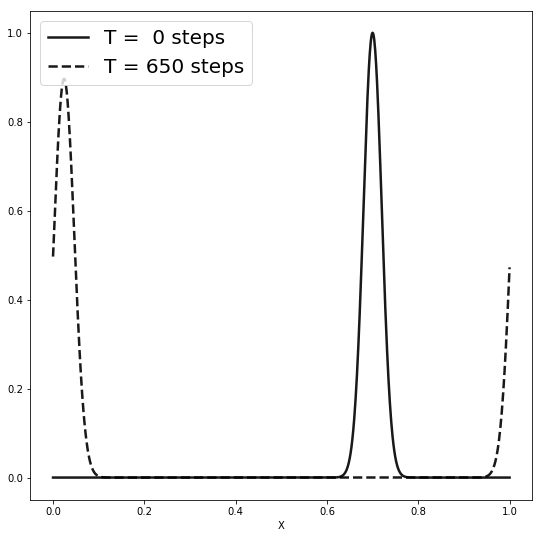
\includegraphics[width=.8\linewidth]{figures/stable_not_realizable.png}
		\caption{}
		\label{fig:sfig1}
	\end{subfigure}%
	\begin{subfigure}{.5\textwidth}
		\centering
		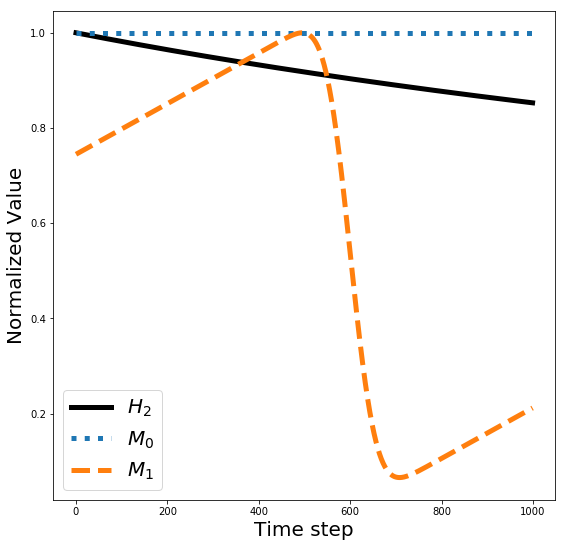
\includegraphics[width=.8\linewidth]{figures/stable_not_real_diagnostic.png}
		\caption{}
		\label{fig:sfig2}
	\end{subfigure}
	\caption{(a) The solution to the Advection-Diffusion equation with periodic boundary conditions after 650 time steps with $\delta = .2$, $\alpha = .5$, parameters that are stable, but not physically realizable. (b) Diagnostic plots confirming that the solution is stable, these values for the different diagnostics were normalized so as to fit on the same plot. Not that $M_1$ is not monotonically increasing as a consequence of the periodic boundary conditions, not a numerical error.}
	\label{fig:fig}
\end{figure}

\section{HW 1 - 1D Diffusion}

In order to efficiently compute the Diffusion equation in 1-D we realize that the transfer matrix T will be described by $T= {\delta, 1-2\delta, \delta}$. If we wish to impose Dirichlet boundary conditions on the simulation then we construct T below with an extra row and column at the extremes of the matrix to keep the edge values unchanged with the iterations.

\begin{equation}
T_{dif}=\begin{bmatrix} 
1       & 0 & 0 &\dots& \dots &0&0 \\
a      & c & b & 0&\dots & 0 &0\\
0& a & c & b & 0 &\dots & 0 \\
\hdotsfor{7} \\
0 &\dots & \dots & 0&a & c & b  \\
0     &0  & 0 & \dots&\dots & 0&1
\end{bmatrix}
\label{eq:T_Diffusion}
\end{equation}
where $a = b =\delta$, and $c=1-2\delta$
If we define $f_n$ as a vector of length NX at time step n then we can commute the state of the system at any time step by performing the operation
\begin{equation}
T^n * f_0 = f_n
\label{eq:diffusion_prop}
\end{equation}


\subsection{Efficiency}
From \cite{matrix_flops} we know that to multiply two N x N matrices together requires $2N^3$ flops. So the flops required to execute Eq. \ref{eq:diffusion_prop} should be $(2*NX^3)*n$ for $T^n$. This should account for the vast majority of the run time, and would predict with my processors max rate of 2.8 GHz a wall clock time of around 
\begin{equation}
	2*100^3*5000 / (2.8 * 10^9) \approx 3 seconds
\end{equation}
for NX = 100, and n = 5000. However, when I run this algorithm using the Numpy (numeric python library) command numpy.linalg.matrix\_power() I find my WCT to be only 5 ms. One unlikely, though pleasant, conclusion we could draw from this is that my cpu is actually operating in 10000 GHz range, unfortunately however, this seems implausible. A more likely explanation is that because T was defined as a tridiagonal matrix there are computational tricks that the Numpy library is using in order to radically reduce the computational cost of raising the matrix to a power. 

\subsection{1-D Diffusion Diagnostics}
\subsubsection{Mass}
Based on our Dirichlet boundary conditions we should not expect mass to be conserved. This is easily seen if we imagine we are simulating heat flow, Dirichlet boundary conditions would mean that our system was embedded in a heat bath, so energy (heat) would not be conserved. This 
is borne out in the simulations I performed. In simulations such as shown in figure \ref{fig:1D_diffu_diri1} where the Dirichlet boundaries had a higher value than the average of the initial condition the total mass, and entropy, of the system increased as time was run forward. The opposite effect occurred, figure \ref{fig:1D_diffu_diri0}, when the boundaries were held at 0, here they sucked mass away from the system and entropy ($H_2$ decreased).  


\begin{figure}
	\begin{subfigure}{.5\textwidth}
		\centering
		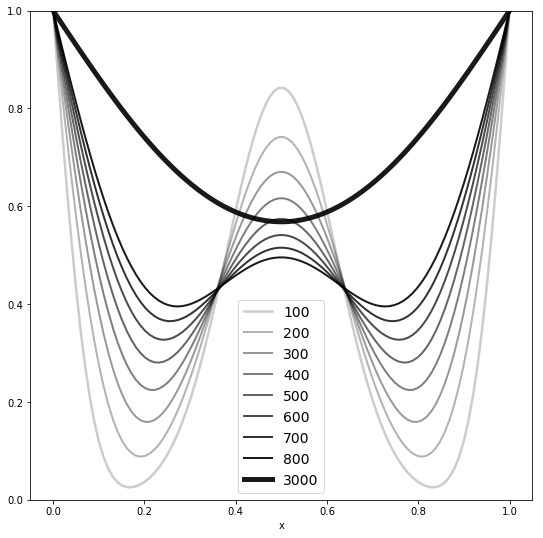
\includegraphics[width=.8\linewidth]{figures/1D_diffusion.png}
		\caption{}
	\end{subfigure}%
	\begin{subfigure}{.5\textwidth}
		\centering
		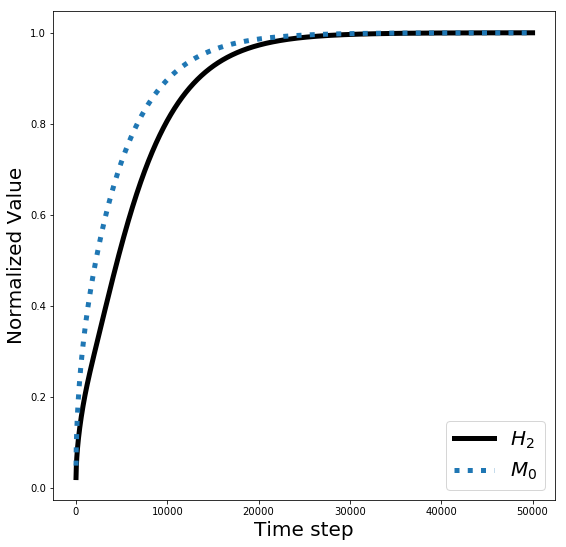
\includegraphics[width=.8\linewidth]{figures/1D_diffusion_diag.png}
		\caption{}
	\end{subfigure}
	\caption{(a)A plot of the results for a simulation of 1 dimensional diffusion with Dirichlet boundary conditions with the edges held at a value of 1. The initial conditions were a sharp Gaussian in the center of the simulation with a max value of one.. The legend refers to the time step at which each curve occurred. The curves are arranged later in time by increasing darkness. (b) Diagnostic plots confirming that the solution is slowly gaining mass and entropy over time. Note however, that the these values do not explode to infinity exponentially as we might expect for an unstable ($\gamma>0$) system. Rather they asymptote to values determined by the Dirichlet boundary conditions.}
	\label{fig:1D_diffu_diri1}
\end{figure}

\begin{figure}
	\begin{subfigure}{.5\textwidth}
		\centering
		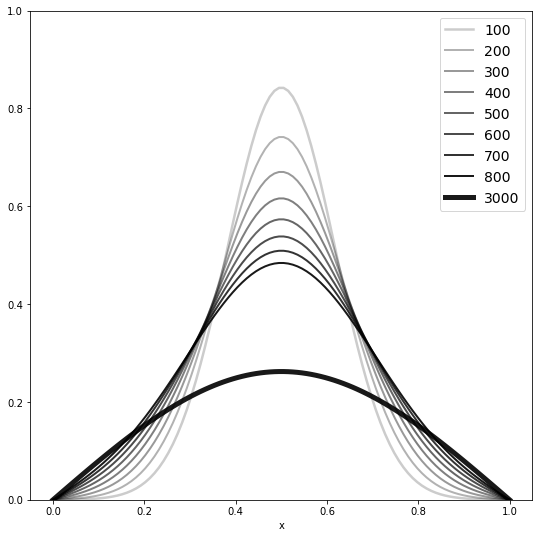
\includegraphics[width=.8\linewidth]{figures/1D_Diffusion_DirBound0.png}
		\caption{}
	\end{subfigure}%
	\begin{subfigure}{.5\textwidth}
		\centering
		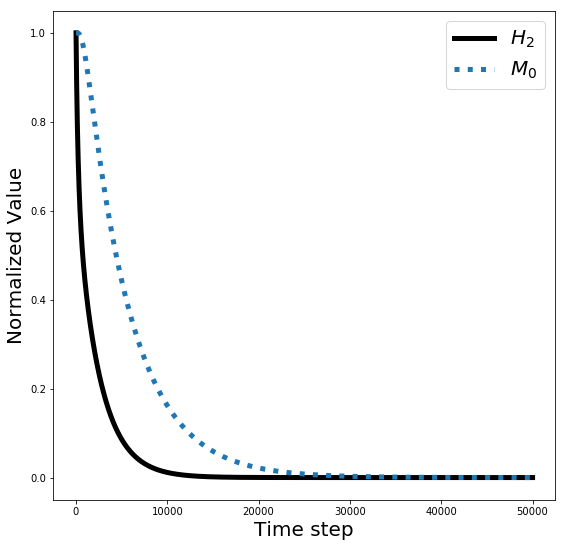
\includegraphics[width=.8\linewidth]{figures/1D_Diffusion_DirBound0_diag.png}
		\caption{}
	\end{subfigure}
	\caption{(a)A plot of the results for a simulation of 1 dimensional diffusion with Dirichlet boundary conditions with the edges held at a value of 1. The initial conditions were a sharp Gaussian in the center of the simulation with a max value of one . (b) Diagnostic plots confirming that the solution is slowly losing mass and entropy over time. Note however, that the these values do not oscillate into negative territory as we might expect for an unstable system. Rather they asymptote to values determined by the Dirichlet boundary conditions.}
	\label{fig:1D_diffu_diri0}
\end{figure}
\subsection{1-D Advection Diffusion}
This is easily extensible to solve the Advection-Diffusion equation, we simply need alternate values for a,b, and c for the definition of $T$, Eq. \ref{eq:diffusion_prop}.
\begin{align}
a = \delta + \frac{\alpha}{2}
c = 1 - 4\delta
b = \delta - \frac{\alpha}{2}
\end{align}

With this redefined T the numerical solution is just as efficient as before though the behavior of the solution, see Figure \ref{fig:1D_AD}, is somewhat more asymmetrical on account of the constant "wind" force provided by Advection.
\begin{figure}
	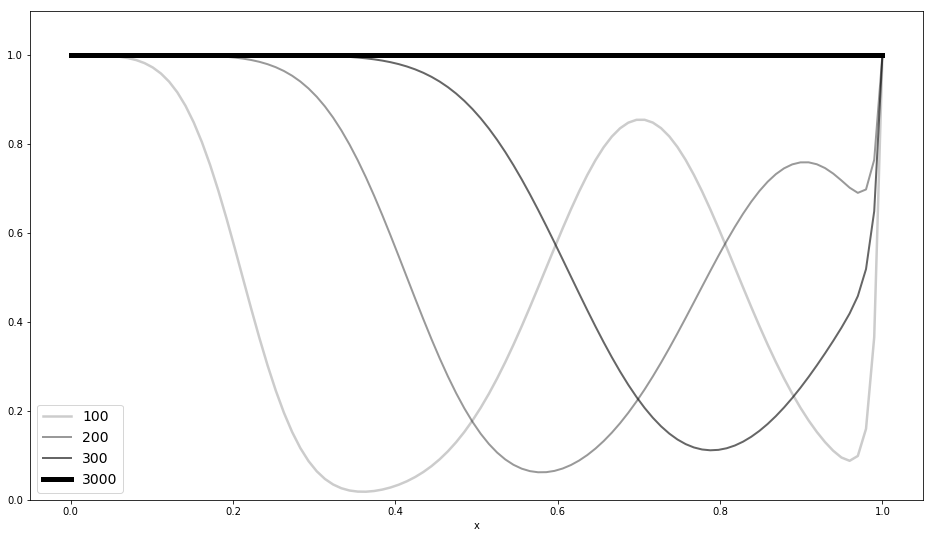
\includegraphics[width=\linewidth]{figures/1D_AD.png}%
	\caption{A plot of the results for a simulation of 1 dimensional diffusion with Dirichlet boundary conditions. The initial conditions were a sharp Gaussian in the centered at .7, with a max value of one, and the two edge points were held to values of 1. In this simulation the space "fills up" from the left as a consequence of the "wind" of Advection. The wind pushes the initial Gaussian into the right wall where it is absorbed and prevents the right side boundary condition from contributing strongly to the rest of the simulated points. As in other plots the legend refers to the time step and darker values indicate a later time step. }
	\label{fig:1D_AD}
\end{figure}


\section{HW 1 - 2D Diffusion with Dirichlet BC}
\label{sec:HW1_2D}
Extending our solution to 2D requires consideration of nearest neighbors in 2 rather than one dimension.  When using the 4 neighbors closely aligned on the grid we need to consider the rules defined by Eq. \ref{eq:dx} and \ref{eq:dx^2} for both spatial dimensions. This ultimately results in a transfer matrix described by $T_{jk} = \{\delta,1-4\delta,\delta\}$. Propagating this forward in time allows us to see the evolution of a system in 2D dimensions as in Figure \ref{fig:2D}
\begin{figure}
	\begin{subfigure}{.5\textwidth}
		\centering
		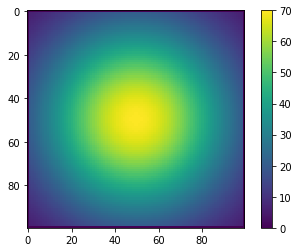
\includegraphics[width=.8\linewidth]{figures/2D_Diffusion_DirBound0_init.png}
		\caption{}
	\end{subfigure}%
	\begin{subfigure}{.5\textwidth}
		\centering
		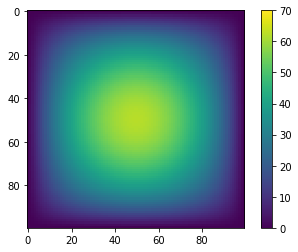
\includegraphics[width=.8\linewidth]{figures/2D_Diffusion_DirBound0_end.png}
		\caption{}
	\end{subfigure}
	\begin{subfigure}{.5\textwidth}
		\centering
		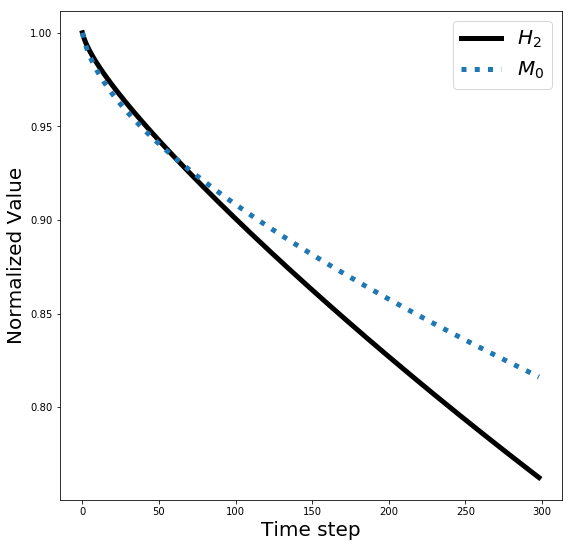
\includegraphics[width=.8\linewidth]{figures/2D_Diffusion_DirBound0.png}
		\caption{}
	\end{subfigure}
	\caption{(a) Initial condition for a simulation of the diffusion equation in 2 dimensions with the boundaries held to a Dirichlet condition at a value of 0. (b) Some time later the system has evolved and the average value is being pulled to zero by the boundary conditions. (c) A diagnostic plot confirms that the solution is slowly losing mass and entropy over time.}
	\label{fig:2D}
\end{figure}
 

\section{HW 2 - 1D Advection Diffusion Reaction }
While we have previously covered the equation of a physical process governed by Advection and Diffusion, the natural addition to that pair is Reaction. Reaction can be thought of as chemistry, or that the nature (or amount) of a substance will change in time even in the absence of both Advection and Diffusion.

The Advection-Diffusion-Reaction is an extension of Equation \ref{eq:AD_cont} with the addition of the operator $R$ describing any chemical processes.
\begin{equation}
\partial_t \varphi = -U \partial_x \varphi + D \partial_{xx}\varphi + R(\varphi).
\label{eq:ADR_cont}
\end{equation}
The operator $R$ can be very simple as in the case of linear chemistry:
\begin{equation}
R(\varphi) = r \varphi, r \in \mathbb{R},
\label{eq:linear_chem}
\end{equation}
or more complicated such as described by the logistic equation:
\begin{equation}
R(\varphi) = a \varphi-b \varphi^2, a,b \in \mathbb{R},
\label{eq:chem_logis}
\end{equation}
which, unlike the linear growth of Eq \ref{eq:linear_chem} has more than $\varphi  n= 0$ as a stable solution. Over a long enough time period the total mass in a problem with linear chemistry will not cease to grow. However, if $a > b > 0$ we can expect the value of $\varphi$ to eventually reach the value of $a$, which would result in a stable solution assuming that the rest of our numerics are stable. 

\subsection{Computing}
Linear chemistry is trivial to add onto the existing methods we have for calculating AD equations. We can use the same matrix as Eq. \ref{eq:T_Diffusion}

\begin{equation}
T_{ADR}=\begin{bmatrix} 
1       & 0 & 0 &\dots& \dots &0&0 \\
a      & c & b & 0&\dots & 0 &0\\
0& a & c & b & 0 &\dots & 0 \\
\hdotsfor{7} \\
0 &\dots & \dots & 0&a & c & b  \\
0     &0  & 0 & \dots&\dots & 0&1
\end{bmatrix}
\label{eq:T_Diffusion_2}
\end{equation}
where $a = \delta +\frac{\alpha}{2}$, $b =\delta-\frac{\alpha}{2}$, and $c=1-2\delta +\kappa$, with $\kappa = r h$. 

The case of logistic chemistry is more complicated, however, we can still use the matrix propagator. We can consider $R$ as an operator and realize that what is relevant for calculating $\hat{\varphi}$ is $R = (a - b \varphi) \cdot h$. With this we can recalculate the matrix needed at each time step through simple matrix addition:
\begin{equation}
T_{AD} + (a - b \varphi) \cdot h * \mathbb{I},
\end{equation}
where $T_{AD}$ is the transfer matrix for pure Advection-Diffusion, and $\mathbb{I}$ is the identity Matrix. $\mathbb{I}$ will of dimension Nx x Nx so the addition should exclude the first and last rows and columns of $T_{AD}$ to keep the periodic boundary conditions. The results of such a propagation scheme can be seen in Figure \ref{1D_ADR}


\begin{figure}
	\begin{subfigure}{.5\textwidth}
		\centering
		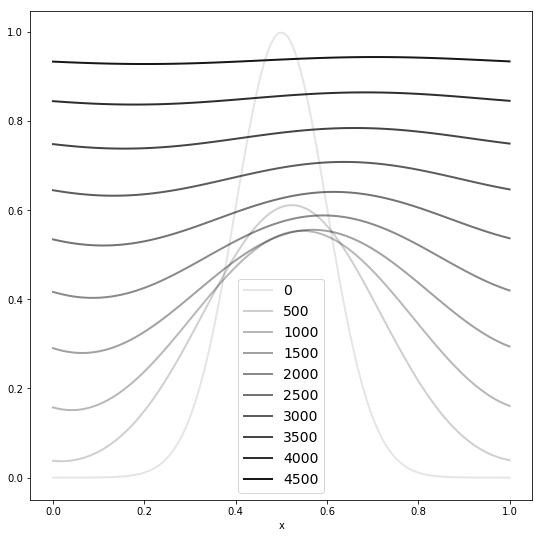
\includegraphics[width=.8\linewidth]{figures/1D_ADR.png}
		\caption{}
	\end{subfigure}%
	\begin{subfigure}{.5\textwidth}
		\centering
		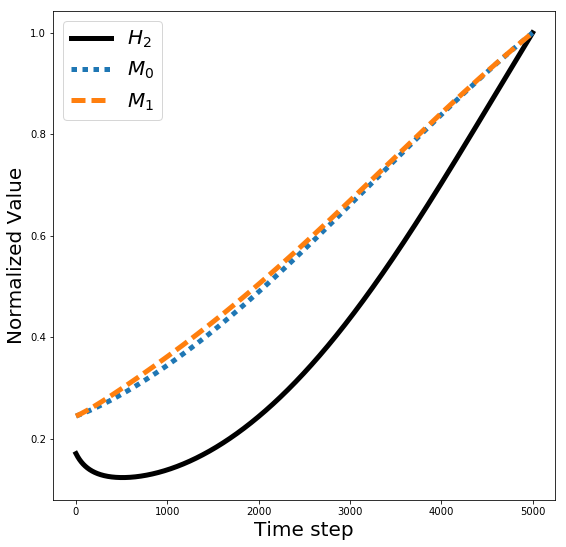
\includegraphics[width=.8\linewidth]{figures/1D_ADR_diag.png}
		\caption{}
	\end{subfigure}
	\caption{(a) A plot of the results for a simulation of 1 dimensional ADR with periodic boundary conditions. The initial condition was a sharp Gaussian in the center of the simulation with a max value of one. (b) Diagnostic plots confirming that the solution is slowly gaining mass and entropy over time. The entropy shows an interesting feature, where at first it decreases, likely due to strong diffusivity, and then grows as there is more mass added to the system due to chemistry. The number of time steps was kept limited here in order to showcase the details at low t, however, if the simulation is extended for a long time the mass asymptotes to the value expected from the logistic chemistry, giving us confidence in the accuracy of our simulation. The diagnostic plots have been normalized so that their maximum value is one.}
	\label{fig:1D_ADR}
\end{figure}

\subsection{Crank- Nicolson}
Another way to propagate chemistry forward in time is to use an iterative time marching method. This method has the advantage of being easy to commute $\mathcal{O}(N*N_{iterations})$ while being fairly stable.
	
For a pure chemistry system we will have:
\begin{equation}
\hat{\varphi} = \varphi + R(\varphi)\cdot h/2 +R(\hat{\varphi})\cdot h/2
\end{equation}
this immediately is a problem as we cannot commute $\hat{\varphi}$ without knowing it first. The solution undertaken in a crank nicolson method is to first commute
\begin{equation}
\varphi^* = \varphi + R(\varphi)*h, 
\end{equation}
which is just the forward Euler result. Then to use the forward Euler results to calculate
\begin{equation}
\hat{\varphi} = \varphi + R(\varphi)\cdot h/2 +R(\hat{\varphi^*})\cdot h/2.
\end{equation}
\begin{figure}
	\begin{subfigure}{.5\textwidth}
		\centering
		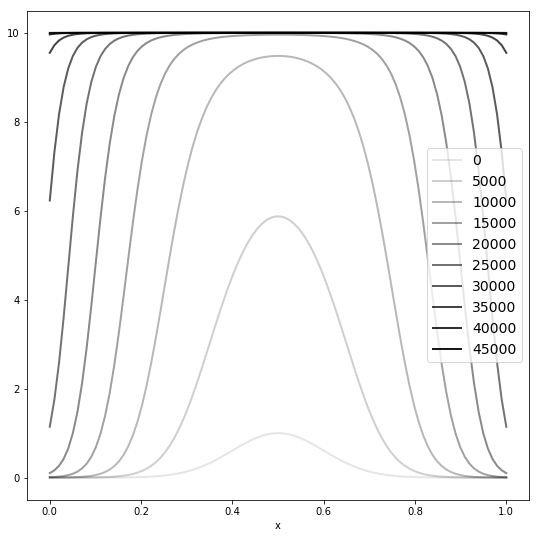
\includegraphics[width=.8\linewidth]{figures/crank_nic_1D.png}
		\caption{}
	\end{subfigure}%
	\begin{subfigure}{.5\textwidth}
		\centering
		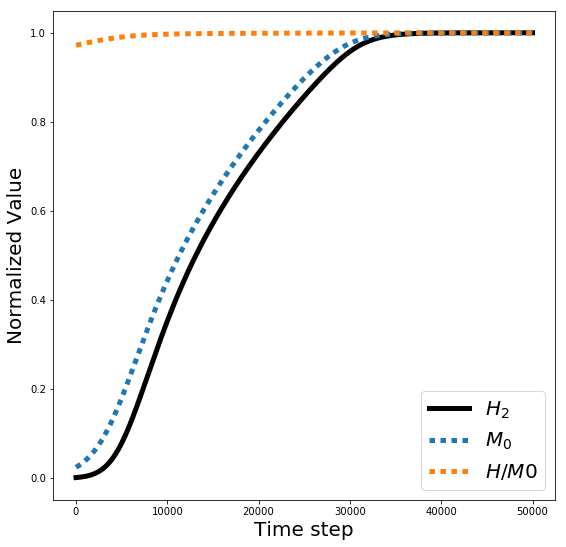
\includegraphics[width=.8\linewidth]{figures/crank_nic_diag.png}
		\caption{}
	\end{subfigure}
	\caption{(a) A plot of the results for a simulation of 1 dimensional chemistry only equation (R) with periodic boundary conditions. The initial condition was a sharp Gaussian in the center of the simulation with a max value of one. Over time the solution appraoches the limiting value we would predict based on the (b) Diagnostic plots confirming that the solution is  gaining mass and entropy over time. The Entropy per unit mass H/M0 fairly quickly approaches its maximum value. The diagnostic plots have been normalized so that their maximum value is one.}
	\label{fig:1D_crank_nic}
\end{figure}

\subsection{Commutability of Chemistry and AD Operators}
In the system of ADR we can split our operator into two separate operators $L_1$ for just AD and $L_2$ for R. We could thus consider that our solution for $\varphi(t+h)$ could be written as either:
\begin{equation}
e^{L_1h}\{e^{(L_2h)}\varphi\} \text{ or } e^{L_2h}\{e^{(L_1h)}\varphi\}.
\end{equation}
However, this will only be true if the operators commute. When considering a system of limited size an easy way to determine the commutation error is to simply attempt both orderings of operators and observe the difference between the two solutions. In Figure \ref{fig:commute_error} we can see that these operators commute extremely well for logistic chemistry, as we might have expected.
\begin{figure}
	\centering
	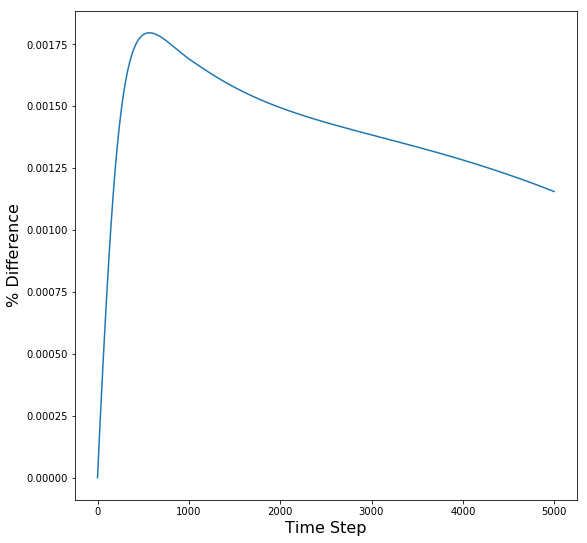
\includegraphics[width=\textwidth]{figures/operator_order_rel_dif.png}
	\caption{A plot of the relative error when propagating and ADR equation in time with different operator error. The values on the Y axis are the average over the simulation grid of the percent difference between the operator orderings. As we expect chemistry and AD to commute well they are correspondingly small.  }
	\label{fig:commute_error}
\end{figure}

\section{HW2 - Adaptive Time Stepping for $\dot{x}=x^2$}
Choosing a time a priori can be difficult in order to achieve a desired level of accuracy in a reasonable amount of computation time. Furthermore, a static $\Delta t$ may be a reasonable value early in the computation but become too large as the system evolves. The solution to this is update $\Delta t$ as the simulation progresses. 

In the case of the following equation:

\begin{equation}
\dot{x} = x^2
\label{eq:ODE_thing}
\end{equation}
we can propagate forward in time by transforming the time derivative to the discrete regime.
\begin{equation}
\frac{\hat{x}-x}{h} = x^2
\end{equation}
\begin{equation}
\hat{x} = hx^2+x.
\end{equation}
Now if we merely want to ensure that we are never jumping too far forward in time then we can limit the growth of the function in any one step. We do this by defining some epsilon as the maximum possible growth in a single time step:
\begin{equation}
|\frac{\hat{x}}{x}-1| < \epsilon,
\end{equation}
plugging in our value of $\hat{x}$ gives us
\begin{equation}
h < \frac{\epsilon}{x}
\end{equation}
as a condition to limit our growth. If we calculate $\frac{\epsilon}{x}$ at every time step then we should update $h$ according to 
\begin{equation}
h = q*\frac{\epsilon}{x},
\end{equation}
where $0<q<1$ is a factor added to ensure our safety in terms of growth. Smaller values of $\epsilon$ should then result in more, smaller, time step and a more accurate solution. As seen in Figure \ref{fig:adaptive}, smaller values of epsilon result in numerical solutions that are closer to the analytic solution of $x(t) = \frac{x(0)}{1-x(0)t}$.

\begin{figure}
	\centering
	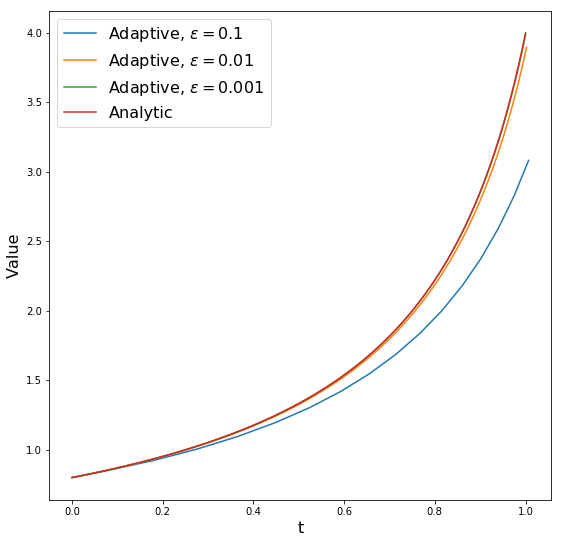
\includegraphics[width=\textwidth]{figures/adaptive.png}
\caption{A plot comparing the analytic solution to Eq. \ref{eq:ODE_thing} to our adaptive method with various values of $\epsilon$. $\epsilon = 0.001$ is on the plot, however, at these scales it is indistinguishable from the analytic solution. For $\epsilon = \{0.1, 0.01, 0.001\}$ the solutions took 17, 178, and 1787 time steps to complete.  }
	\label{fig:adaptive}
\end{figure}
\section{Summary}
In this work I derived the dispersion relation for the discrete version of the Advection-Diffusion equation and analyzed its numerical stability, find that we require $\alpha^2 < 2\delta$ is necessary for stability but not sufficient to have a physically realizable solution. Following this I implemented a numerical solver for the 1 and 2 Dimensional Diffusion equations and examined several diagnostics. This analysis revealed that the boundary conditions are very important.

We have also considered the addition of chemistry to the Advection Diffusion equation and implemented three different methods of solving it. Namely, forward Euler, crank-nicolson, and forward Euler with operator splitting. An adaptive time stepping method for solving ODE's was also considered. 
 
\section{Acknowledgements}
I consulted with Jenny Coulter for the sections in this document for HW 1. 

  \begin{thebibliography}{1}
  	
  	\bibitem{matrix_flops} D. Olesky, Matrix Multiplication, Flop Counts and Block (Partitioned) Matrices, http://webhome.csc.uvic.ca/~dolesky/csc449-540/1.1-1.2.pdf

  \end{thebibliography}



\end{document}
